\documentclass[oneside,numbers,spanish]{ezthesis}
%% # Opciones disponibles para el documento #
%%
%% Las opciones con un (*) son las opciones predeterminadas.
%%
%% Modo de compilar:
%%   draft            - borrador con marcas de fecha y sin im'agenes
%%   draftmarks       - borrador con marcas de fecha y con im'agenes
%%   final (*)        - version final de la tesis
%%
%% Tama'no de papel:
%%   letterpaper (*)  - tama'no carta (Am'erica)
%%   a4paper          - tama'no A4    (Europa)
%%
%% Formato de impresi'on:
%%   oneside          - hojas impresas por un solo lado
%%   twoside (*)      - hijas impresas por ambos lados
%%
%% Tama'no de letra:
%%   10pt, 11pt, o 12pt (*)
%%
%% Espaciado entre renglones:
%%   singlespace      - espacio sencillo
%%   onehalfspace (*) - espacio de 1.5
%%   doublespace      - a doble espacio
%%
%% Formato de las referencias bibliogr'aficas:
%%   numbers          - numeradas, p.e. [1]
%%   authoryear (*)   - por autor y a'no, p.e. (Newton, 1997)
%%
%% Opciones adicionales:
%%   spanish         - tesis escrita en espa'nol
%%
%% Desactivar opciones especiales:
%%   nobibtoc   - no incluir la bibiolgraf'ia en el 'Indice general
%%   nofancyhdr - no incluir "fancyhdr" para producir los encabezados
%%   nocolors   - no incluir "xcolor" para producir ligas con colores
%%   nographicx - no incluir "graphicx" para insertar gr'aficos
%%   nonatbib   - no incluir "natbib" para administrar la bibliograf'ia

%% Paquetes adicionales requeridos se pueden agregar tambi'en aqu'i.
%% Por ejemplo:
%\usepackage{subfig}
%\usepackage{multirow}

%% # Datos del documento #
%% Nota que los acentos se deben escribir: \'a, \'e, \'i, etc.
%% La letra n con tilde es: \~n.

\author{Raul Edgar Quispe Totocayo }
\title{Comparaci\'on de GCD}
%\degree{Doctor en Ciencias}
%\supervisor{Nombre de mi Asesor}
\institution{Universidad Nacional de San Agustin}
\faculty{Escuela Profesional de Ciencia de la Computaci\'on \\ \small{\LaTeX{}}}
%\department{Departamento de Sistemas Computacionales}

%% # M'argenes del documento #
%% 
%% Quitar el comentario en la siguiente linea para austar los m'argenes del
%% documento. Leer la documentaci'on de "geometry" para m'as informaci'on.

%\geometry{top=40mm,bottom=33mm,inner=40mm,outer=25mm}

%% El siguiente comando agrega ligas activas en el documento para las
%% referencias cruzadas y citas bibliogr'aficas. Tiene que ser *la 'ultima*
%% instrucci'on antes de \begin{document}.
\usepackage[utf8]{inputenc}
\usepackage{amsmath}
\usepackage{tikz}
\usepackage{dsfont}
\usepackage{textcomp}
\usepackage{float}
\usepackage{amssymb,amsthm,amsfonts,latexsym,cancel}
\usepackage{graphicx}
\usepackage{listings}
\usepackage{algorithm}
\usepackage{color}
\usepackage{longtable}
\usepackage{rotating}
\usepackage{subfigure}

\definecolor{gray97}{gray}{.97}
\definecolor{gray75}{gray}{.75}
\definecolor{gray45}{gray}{.45}
\lstset{ frame=Ltb,
     framerule=0pt,
     aboveskip=0.5cm,
     framextopmargin=3pt,
     framexbottommargin=3pt,
     framexleftmargin=0.4cm,
     framesep=0pt,
     rulesep=.4pt,
     backgroundcolor=\color{gray97},
     rulesepcolor=\color{black},
     %
     stringstyle=\ttfamily,
     showstringspaces = false,
     basicstyle=\small\ttfamily,
     commentstyle=\color{gray45},
     keywordstyle=\bfseries,
     %
     numbers=left,
     numbersep=15pt,
     numberstyle=\tiny,
     numberfirstline = false,
     breaklines=true,
   }

% minimizar fragmentado de listados
\lstnewenvironment{listing}[1][]
   {\lstset{#1}\pagebreak[0]}{\pagebreak[0]}

\lstdefinestyle{consola}
   {basicstyle=\scriptsize\bf\ttfamily,
    backgroundcolor=\color{gray75},
    }
\lstdefinestyle{C}
   {language=C,
   }
\hyperlinking

\begin{document}

%% En esta secci'on se describe la estructura del documento de la tesis.
%% Consulta los reglamentos de tu universidad para determinar el orden
%% y la cantidad de secciones que debes de incluir.

%% # Portada de la tesis #
%% Mirar el archivo "titlepage.tex" para los detalles.
%% ## Construye tu propia portada ##
%% 
%% Una portada se conforma por una secuencia de "Blocks" que incluyen
%% piezas individuales de informaci'on. Un "Block" puede incluir, por
%% ejemplo, el t'itulo del documento, una im'agen (logotipo de la universidad),
%% el nombre del autor, nombre del supervisor, u cualquier otra pieza de
%% informaci'on.
%%
%% Cada "Block" aparece centrado horizontalmente en la p'agina y,
%% verticalmente, todos los "Blocks" se distruyen de manera uniforme 
%% a lo largo de p'agina.
%%
%% Nota tambi'en que, dentro de un mismo "Block" se pueden cortar
%% lineas usando el comando \\
%%
%% El tama'no del texto dentro de un "Block" se puede modificar usando uno de
%% los comandos:
%%   \small      \LARGE
%%   \large      \huge
%%   \Large      \Huge
%%
%% Y el tipo de letra se puede modificar usando:
%%   \bfseries - negritas
%%   \itshape  - it'alicas
%%   \scshape  - small caps
%%   \slshape  - slanted
%%   \sffamily - sans serif
%%
%% Para producir plantillas generales, la informaci'on que ha sido inclu'ida
%% en el archivo principal "tesis.tex" se puede accesar aqu'i usando:
%%   \insertauthor
%%   \inserttitle
%%   \insertsupervisor
%%   \insertinstitution
%%   \insertdegree
%%   \insertfaculty
%%   \insertdepartment
%%   \insertsubmitdate

\begin{titlepage}
  \TitleBlock[\bigskip]{\Huge\scshape\insertfaculty}
  \TitleBlock{\Huge\scshape\inserttitle}
  \begin{center}
      
\includegraphics[scale=0.2]{pictures/chunsa.png}
  % chunsa.png: 0x0 pixel, 300dpi, 0.00x0.00 cm, bb=
  \end{center}
  \TitleBlock{\scshape\insertauthor}
    %Tesis presentada por \insertauthor \\
    %para obtener el grado de \insertdegree}
  \TitleBlock{\insertsubmitdate}
  %\TitleBlock[\bigskip]{\insertdepartment}
\end{titlepage}

%% Nota 1:
%% Se puede agregar un escudo o logotipo en un "Block" como:
%%   \TitleBlock{\includegraphics[height=4cm]{escudo_uni}}
%% y teniendo un archivo "escudo_uni.pdf", "escudo_uni.png" o "escudo_uni.jpg"
%% en alg'un lugar donde LaTeX lo pueda encontrar.

%% Nota 2:
%% Normalmente, el espacio entre "Blocks" se extiende de modo que el
%% contenido se reparte uniformemente sobre toda la p'agina. Este
%% comportamiento se puede modificar para mantener fijo, por ejemplo, el
%% espacio entre un par de "Blocks". Escribiendo:
%%   \TitleBlock{Bloque 1}
%%   \TitleBlock[\bigskip]{Bloque2}
%% se deja un espacio "grande" y de tama~no fijo entre el bloque 1 y 2.
%% Adem'as de \bigskip est'an tambi'en \smallskip y \medskip. Si necesitas
%% aun m'as control puedes usar tambi'en, por ejemplo, \vspace*{2cm}.




%% # Prefacios #
%% Por cada prefacio (p.e. agradecimientos, resumen, etc.) crear
%% un nuevo archivo e incluirlo aqu'i.
%% Para m'as detalles y un ejemplo mirar el archivo "gracias.tex".
%\include{gracias}

%% # 'Indices y listas de contenido #
%% Quitar los comentarios en las lineas siguientes para obtener listas de
%% figuras y cuadros/tablas.
\tableofcontents
%\listoffigures
\listoftables

%% # Cap'itulos #
%% Por cada cap'itulo hay que crear un nuevo archivo e incluirlo aqu'i.
%% Mirar el archivo "intro.tex" para un ejemplo y recomendaciones para
%% escribir.
%\include{intro}

\chapter{Algoritmo de Euclides clasico}

\section{Definici\'on}
El algoritmo de Euclides es un m\'etodo antiguo y eficaz para calcular el m\'aximo com\'un divisor (MCD). Fue originalmente descrito por Euclides en su obra Elementos.este algoritmo consiste en : \\
1.Si b=0 entonces maximoComunDivisor(a,b)=a y termina el algortimo\\
2.En otro caso maximoComunDivisor(a,b)=maximoComunDivisor(b,r) donde r es el resto al dividir a entre b.Para calcular maximoComunDivisor(b,r) se utilizan las mismas reglas \\

\section{Algoritmo}
Recordemos que $\:mod(a, b)$ denota el resto de la división de a por b. En este algoritmo, en cada paso $\:r = mod (rn+1, rn)$ donde $\:rn+1 = c$ es el dividendo actual y $\:rn = d$ es el divisor actual.
Luego se actualiza $\:rn+1 = d$ y $d = r$. El proceso continúa mientras d no se anule.\\
Datos: $\:a,b \in Z\:/b\neq0$\\
Salida: $mcd(a,b)$\\
\begin{equation}
 \begin{align}
  c=&|a|,d=|b|;\\
  while&\:d\neq0\:do\\
  r&=mod(c,d);\\
  c&=d;\\
  d&=r;\\
  return&\:mcd(a,b)=|c|;
 \end{align}
\end{equation}
\section{Seguimiento del codigo}
\begin{table}[H]
\label{tablax}
\begin{center}
\begin{tabular}{|c|c|c|c|}
\hline 
a&b&q&r \\
\hline
957349573453465&8346583456&114699&4797633721\\\hline
8346583456&4797633721&1&3548949735\\\hline
4797633721&3548949735&1&1248683986\\\hline
3548949735&1248683986&2&1051581763\\\hline
1248683986&1051581763&1&197102223\\\hline
1051581763&197102223&5&66070648\\\hline
197102223&66070648&2&64960927\\\hline
66070648&64960927&1&1109721\\\hline
64960927&1109721&58&597109\\\hline
1109721&597109&1&512612\\\hline
597109&512612&1&84497\\\hline
512612&84497&6&5630\\\hline
84497&5630&15&47\\\hline
5630&47&119&37\\\hline
47&37&1&10\\\hline
37&10&3&7\\\hline
10&7&1&3\\\hline
7&3&2&1\\\hline
3&1&3&0\\\hline
\end{tabular}
\end{center}
\caption{seguimiento de codigo}
\end{table}


\section{Implementacion del algoritmo}
\begin{lstlisting}[language=C++]
ZZ euclides(ZZ a, ZZ b)//
{
    ZZ q,r;
    q=a/b;
    //r=module(a,b);
    r=a%b;
    while(r!=0)
    {
        q=a/b;
        //r=module(a,b);
        r=a%b;
        a=b;
        b=r;
    }
    return r;
}
\end{lstlisting}
%clasico
\chapter{Algoritmo de Menor Resto}
\section{Definición}
es muy apropiada para fines teóricos. Que el resto sea
positivo es adecuado, como vimos, para mostrar unicidad.
Sin embargo el resto no tiene porque ser positivo, por ejemplo si a = 144 y b = 89,
\begin{itemize}
    \item 144 = 89 · 1 + 55, resto r2 = $55 < b = 89$
    \item 144 = 89 · 2 − 34, resto r1 = $34 < b = 89$

\end{itemize}

\section{Implementacion del algoritmo}
\begin{lstlisting}[language=C++]
#include <iostream>
#include <NTL/ZZ.h>//includ  the lib ntl 
#include <ctime>
#include <fstream>
using namespace std;//using std namespace 
using namespace NTL;//using NTL namespaces
unsigned t0,t1;

ZZ module(ZZ &x,ZZ &y){
    ZZ q=x/y,r;
    if(q<0)
    {
        q=-1*q;
        q++;
        q=-1*q;
        r=x-(q*y);
    }
    else 
    {
        r=x-(q*y);
    }
    return r;
}
ZZ menor(ZZ x,ZZ y)
{
    if(y<x)
        return y;
    else 
        return x;
}
void euclides(ZZ a, ZZ b)//
{
    //t0=clock();
    ZZ q,q1,r;
    q=a/b;
    q1=q;q1++;
    r=menor(a-(q*b),a-(q1*b));
    //r=a%b;
    while(r!=0)
    {
        q=a/b;
        q1=q;q++;
        r=menor(a-(q*b),a-(q1*b));
        //cout << a  << '\t'<<  " = " << q << "(" << b << ")" << "+" << r << endl;//print the euclides algorithm
        a=b;
        b=r;
    }
    cout << "result is "<< a << endl;
    //t1=clock();
}
//funcion para guardar los datos 
int main()
{
    ZZ a,b;
    cout << "input a:" ; cin >> a; //imput the numbers 
    cout << "input b:" ; cin >> b;
    euclides(a,b);
    //double time=(double(t1-t0)/CLOCKS_PER_SEC);
    //cout << "Execution time:" << time << endl;

}
\end{lstlisting}
\section{Seguimiento del codigo}
\begin{table}[H]
\label{tablax}
\begin{center}
\begin{tabular}{|c|c|c|c|}
\hline 
a&b&q&r \\
\hline
9792347293422342&10048&974592347234&-356611584890\\\hline
974592347234&-2&-356611584890&-95242407436\\\hline
-356611584890&4&-95242407436&-70884362582\\\hline
-95242407436&2&-70884362582&-24358044854\\\hline
-70884362582&3&-24358044854&-22168272874\\\hline
-24358044854&2&-22168272874&-2189771980\\\hline
-22168272874&11&-2189771980&-270553074\\\hline
-2189771980&9&-270553074&-25347388\\\hline
-270553074&11&-25347388&-17079194\\\hline
-25347388&2&-17079194&-8268194\\\hline
-17079194&3&-8268194&-542806\\\hline
-8268194&16&-542806&-126104\\\hline
-542806&5&-126104&-38390\\\hline
-126104&4&-38390&-10934\\\hline
-38390&4&-10934&-5588\\\hline
-10934&2&-5588&-5346\\\hline
-5588&2&-5346&-242\\\hline
-5346&23&-242&-22\\\hline
-242&12&-22&0\\\hline
\end{tabular}
\end{center}
\caption{seguimiento de codigo}
\end{table}%menor resto
\chapter{Algoritmo Euclides Extendido}
\section{Definición}
El algoritmo de Euclides extendido permite, además de encontrar un máximo común divisor de dos números enteros  $a\: y\: b$, expresarlo como la mínima combinación lineal de esos números, es decir, encontrar números enteros $s\: y\: t$ tales que $mcd(a,b)=as+bt$. Esto se generaliza también hacia cualquier dominio euclideano.
\section{El algoritmo de Euclides Extendido}
\subsection{Fundamentos}
\begin{itemize}
 \item Usar el algoritmo tradicional de Euclides. En cada paso, en lugar de a dividido entre b es q y de resto r se escribe la ecuación $a = b q + r$
 \item Se despeja el resto de cada ecuación.
 \item Se sustituye el resto de la última ecuación en la penúltima, y la penúltima en la antepenúltima y así sucesivamente hasta llegar a la primera ecuación, y en todo paso se expresa cada resto como combinación lineal.
\end{itemize}
\section{Implementación}
\begin{lstlisting}[language=C++]
ZZ euclides(ZZ &a, ZZ &b)//
{
    ZZ q,r,r1=a,r2=b,s,s1,s2,t,t1,t2;
    s1=1,s2=0,t,t1=0,t2=1;
    while(r2>0)
    {
        q=r1/r2;
        r=r1-(q*r2);
        r1=r2;
        r2=r;
        //-----
        s=s1-(q*s2);
        s1=s2;
        s2=s;
        t=t1-(q*t2);
        t1=t2;
        t2=t;
    }
    return s1;
}
\end{lstlisting}
\section{Seguimiento del algoritmo}
%\begin{center}
\begin{sideways}
\begin{tabular}{|c|c|c|c|c|c|c|c|c|c|}
\hline
q&r1&r2&r&s1&s2&s&t1&t2&t \\\hline
9998111&93475&70209&70209&0&1&1&1&-9998111&-9998111\\\hline
1&70209&23266&23266&1&-1&-1&-9998111&9998112&9998112\\\hline
3&23266&411&411&-1&4&4&9998112&-39992447&-39992447\\\hline
56&411&250&250&4&-225&-225&-39992447&2249575144&2249575144\\\hline
1&250&161&161&-225&229&229&2249575144&-2289567591&-2289567591\\\hline
1&161&89&89&229&-454&-454&-2289567591&4539142735&4539142735\\\hline
1&89&72&72&-454&683&683&4539142735&-6828710326&-6828710326\\\hline
1&72&17&17&683&-1137&-1137&-6828710326&11367853061&11367853061\\\hline
4&17&4&4&-1137&5231&5231&11367853061&-52300122570&-52300122570\\\hline
4&4&1&1&5231&-22061&-22061&-52300122570&220568343341&220568343341\\\hline
4&1&0&0&-22061&93475&93475&220568343341&-934573495934&-934573495934\\\hline
\end{tabular}
\end{sideways}
%\end{center}


%
%\end{table}




%extendido
\chapter{Algoritmo Binario de Euclides}
\section{Definición}
El algorirmo binario de GCD , tambien conociddo  como algortimo de stein es un algoritmo que calcula el mayor divisor común de dos enteros no negativos.
El algoritmo de Stein utiliza operaciones aritméti-
cas más simples que el algoritmo euclidiano conven-
cional; Reemplaza la división por cambios aritméti-
cos, comparaciones y sustracciones. Aunque el al-
goritmo fue publicado por primera vez por el fı́sico
y programador israelı́ Josef Stein en 1967, [2] puede
haber sido conocido en la China del siglo I.
Opera con los siguientes teoremas
\section{el algoritmo de binario gcd}
\begin{itemize}
 \item Si a,b son pares, $mcd(a,b) = 2 mcd(a/2,b/2)$.
 \item Si a es par y b impar o viceversa, $mcd(a,b) = mcd(a/2,b)\: o\: mcd(a, b/2)$.
 \item Si a,b son impares , $mcd(a,b) = mcd(|a-b|/2, r)$, donde $r = min{a,b}$;
\end{itemize}
\section{Implementación}
\begin{lstlisting}[language=C++]

ZZ binary_gcd( ZZ u,ZZ v)
{
  int i;
  if (u == 0) return v;
  if (v == 0) return u;
  cout << "a" << '\t' << "b" <<'\t' << "i" <<  endl;
  for (i = 0; ((u | v) & 1) == 0; ++i) {
         u >>= 1;
         v >>= 1;
        //cout << u << '\t' << v << '\t' << i <<  endl;      
  }

  while ((u & 1) == 0)
    u >>= 1;
    
  do {
       //cout << u << '\t' << v <<'\t' << i <<  endl;
       while ((v & 1) == 0)  
           v >>= 1;
       if (u > v) {
          ZZ t = v; v = u; u = t;}  
       v = v - u;                       
     } while (v != 0);
  return u << i;
}
\end{lstlisting}
\section{Seguimiento del algoritmo}
\begin{table}[H]
\label{tablax}
\begin{center}
\begin{tabular}{|c|c|c|}
\hline 
a&b&t \\
\hline
843563845&34534&0\\\hline
17267&843546578&0\\\hline
17267&421756022&0\\\hline
17267&210860744&0\\\hline
17267&26340326&0\\\hline
17267&13152896&0\\\hline
17267&85490&0\\\hline
17267&25478&0\\\hline
12739&4528&0\\\hline
283&12456&0\\\hline
283&1274&0\\\hline
283&354&0\\\hline
177&106&0\\\hline
53&124&0\\\hline
31&22&0\\\hline
11&20&0\\\hline
5&6&0\\\hline
3&2&0\\\hline
1&2&0\\\hline
\end{tabular}
\end{center}
\caption{seguimiento de codigo}
\end{table}



%binario
\chapter{left-shift binary algorithm}
\section{Definición}
Este algoritmo debe su nombre al hecho de que se hace multiplicación por 2. En representación
binaria el efecto de multiplicar por dos es un desplazamiento (en una posición), de la representación
binaria original, hacia la izquierda.

\section{Implementacion del algoritmo}
\begin{lstlisting}[language=C++]
#include <iostream>
#include <cmath>
#include <ctime>
#include <fstream>
#include <NTL/ZZ.h>
using namespace std;
using namespace NTL;
unsigned t0,t1;
void guardar(ZZ a,ZZ b,ZZ times,ZZ aux, ZZ s)
{
    ofstream archivo;
    archivo.open("lsbgcd.csv",ios::app);
    archivo << a <<"&"<< b<<"&"<<times<<"&"<< aux<<"&"<<s << "\\\\\\hline"<< endl;
    archivo.close();
}

ZZ menor(ZZ x,ZZ y)
{
    if(y<x)
        return y;
    else 
        return x;
}
ZZ potencia(ZZ a,ZZ b)
{
    ZZ result;
    result=1;
    for (int i = 0; i < b; i++)
    {
         result=a*result;
    }
    return result;
}
ZZ  lsbgcd(ZZ u, ZZ v)
{
    ZZ a,b,t,aux,s,two;
    two=2;
    a=abs(u);
    b=abs(v);
    cout << "a" << '\t'<< '\t' << "b" << '\t'<< '\t' << "t" << '\t'<< '\t' << "aux" << '\t'<< '\t' << "s" << endl;
    while(b!=0)
    {
        s=0;
        while(b*potencia(two,s)<=a)
        {
            s=s+1;
        }
        s=s-1;
        t=menor(a-b*potencia(two,s),b*potencia(two,s+1)-a);
        a=b;
        b=t;
        if(a<b)
        {
            aux=a;
            a=b;
            b=aux;
        }
        cout << a << '\t'<< '\t' << b << '\t'<< '\t' << t << '\t' << '\t'<< aux << '\t'<< '\t' << s <<endl; 
        guardar(a,b,t,aux,s);
    }   
    return a;
}
//save data 
int main()
{
    ZZ a,b;
    cout << "input a:" ; cin >> a; //imput the numbers 
    cout << "input b:" ; cin >> b;
    lsbgcd(a,b);   
}
\end{lstlisting}
\section{Seguimiento del codigo}
\begin{table}[H]
\label{tablax}
\begin{center}
\begin{tabular}{|c|c|c|c|c|}
\hline 
a&b&t&aux&s \\
\hline
51459615586&94237394&51459615586&94237394&13\\\hline
3210069858&94237394&3210069858&94237394&9\\\hline
194473250&94237394&194473250&94237394&5\\\hline
94237394&5998462&5998462&94237394&1\\\hline
5998462&1737998&1737998&94237394&3\\\hline
1737998&953530&953530&94237394&1\\\hline
953530&169062&169062&94237394&0\\\hline
277282&169062&277282&169062&2\\\hline
169062&60842&60842&169062&0\\\hline
60842&47378&47378&169062&1\\\hline
47378&13464&13464&169062&0\\\hline
13464&6478&6478&169062&1\\\hline
6478&508&508&169062&1\\\hline
1650&508&1650&508&3\\\hline
508&382&382&508&1\\\hline
382&126&126&508&0\\\hline
126&122&122&508&1\\\hline
122&4&4&508&0\\\hline
6&4&6&4&4\\\hline
4&2&2&4&0\\\hline
2&0&0&4&1\\\hline
\end{tabular}
\end{center}
\caption{seguimiento de codigo}
\end{table}
%binario
\chapter{Algoritmo Lehmer GCD}

\section{Algoritmo}
El algoritmo de MCD extendido de Lehmer D. H.
Lehmer propuso en un algoritmo dirigido a optimi-
zar el cálculo del máximo común divisor (MCD) de
dos enteros positivos de múltiple precisión utilizan-
do mayormente operaciones de precisión simple, lo
que permite utilizar en la mayor parte de los casos
operaciones internas del procesador. Este algoritmo
puede extenderse de manera directa a un algoritmo
de MCD extendido, aplicable para encontrar la in-
versa modular de sólo un dı́gito. Además, observó
que el proceso subyacente en el algoritmo de Eucli-
des es la aplicación de sucesivas transformaciones
lineales:
\begin{itemize}
 \item[1] While y $\geq$ b do the following:
 \begin{itemize}
  \item[1.1] Set x\_, y\_ to be the high-order digit of x, y, respectively (y\_ could be 0)
  \item[1.2] $A\leftarrow1$, $B\leftarrow0$, $C\leftarrow0$, $D\leftarrow1$ 
  \item[1.3] If ($grupos\_x == grupos\_y$) esto se agregó al algoritmo del presente libro 
  \item[1.4] While ($y\_ + C$) $!= 0$ and $(y\_ + D)!= 0$ do the following:
  \begin{itemize}
   \item $q\leftarrow (x\_ + A)/(y\_ + C)$ , $q\_ \leftarrow (x\_ + B)/(y\_+ D)$ 
   \item if $q = q\_$ then go to step 1.5
   \item $t \leftarrow A-qC, A \leftarrow C, C \leftarrow t, t\leftarrow B - qD, B\leftarrow D, D\leftarrow t$ 
   \item $t\leftarrow x\_ - qy\_, x\_\leftarrow y\_, y\_\leftarrow t$
  \end{itemize}
  \item[1.5] If $B = 0$, then $T \leftarrow x mod y$, $x\leftarrow y, y\leftarrow T$ 
  \item otherwise, $T\leftarrow Ax + By, u\leftarrow Cx + Dy, x\leftarrow T , y\leftarrow u$ \\
 \end{itemize}
 \item[2] Compute $v = gcd(x, y)$ using Algorithm 2.104 
 \item[3] Return(v)
\end{itemize}

\section{Implementaci\'on}
\begin{lstlisting}[language=C++]
#include <iostream>
#include <limits.h>
#include <NTL/ZZ.h>
#include <fstream>
#define MAX_POTENCIAS 3 // para generar un arreglo de potencias de la base
#include <module.h>//this is my library Module 
using namespace std;
using namespace NTL;
void lehmer_gcd(ZZ x, ZZ y);
ZZ enuclides( ZZ a,  ZZ b);
void guardar(int a,int b,int times,int resultado,int x,int y)
{
    ofstream archivo;
    //string line = "\\\\hline";
    archivo.open("lehmer.csv",ios::app);
    archivo << a <<"&"<< b<<"&"<<times <<"&" << resultado<<"&" << x <<"&" << y <<  "\\\\\\hline"<<endl;
    archivo.close();
}
int main()
{
    double segs;
    ZZ x = 565642334;
    ZZ y = 24423424;

    cout << "Aplicando Lehmer, gcd(" << x << ',' << y << ")\n";
    lehmer_gcd(x,y);

    int dj;
    clock_t t_ini = clock();
    dj = euclides(x,y);
    clock_t t_fin = clock();
    cout << dj << " en " << (double)(t_fin - t_ini)*1000.0 / CLOCKS_PER_SEC;
    return 0;

}

ZZ *genera_array_base(ZZ base);
ZZ digitos_base(ZZ num, ZZ arr[], ZZ &grupos);

void lehmer_gcd(ZZ x, ZZ y)
{
    clock_t t_ini = clock();

    ZZ x_, y_, a, b, c, d;
    ZZ q, q_, t, tt, u;
    ZZ grupos_x;
    ZZ grupos_y;
    ZZ base = 1000; // determina un arreglo de potencias de la base.
    ZZ length_bits = sizeof(int)*CHAR_BIT;
    ZZ *arr_potencias = genera_array_base(base); // se crea un array con las potencias de la base.
                                       // si es base 2 se trata de una forma especial (moviendo bits)
    while(y >= base){

        x_ = digitos_base(x, arr_potencias, grupos_x ); // x_ tendrá los dígitos más significativos que unidos serán <= a la base.
                              // la función usa búsqueda binaria en el array de potencias  de la base
        y_ = digitos_base(y, arr_potencias, grupos_y);
	
        a = 1; b = 0; c = 0; d = 1;
        if(grupos_x == grupos_y){ //necesario pues en la siguiente vuelta hay que asegurar que x e y tengan la misma cantidad d cifras
            while( ((y_+c) != 0) && ((y_+d) != 0) ){
                q = (x_+a) / (y_+c);
                q_ = (x_+b)/ (y_+d);
                if (q != q_){
                    break;
                }
                t=a-q*c;
                a = c;
                c = t;
                t = b - q*d;
                b = d;
                d = t;
                t = x_ - q*y_;
                x_ = y_;
                y_ = t;
                guardar(x_,y_,a,b,c,d);
            }
            
        }
        if (b == 0){
            tt = x%y;
            x = y;
            y = tt;
        }
        else{
            tt = a*x + b*y;
            u = c*x + d*y;
            x = tt;
            y = u;
        }
    }

    clock_t t_fin = clock();

    cout << "Lehmer redujo a gcd(" << x << ',' << y << ") en ";
    double segs = (double)(t_fin - t_ini) / CLOCKS_PER_SEC;
    cout << segs * 1000.0 << " milisegundos. \n" << '\n';

    cout << "euclide  gcd(" << x << ',' << y << ") = ";

    t_ini = clock();
    ZZ v = euclides(x,y);
    t_fin = clock();
    cout << v << '\n';
    segs += (double)(t_fin - t_ini) / CLOCKS_PER_SEC;
    cout << "\nTiempo total:" << segs * 1000.0 << " milisegundos" << '\n';
}

ZZ *genera_array_base(ZZ base)
{
    //repetir el primer y último elemento para
    //  retornar lo deseado en la busq. binaria
    //  así se agregan dos elementos más
    ZZ *arr = new ZZ[MAX_POTENCIAS+2];

    arr[0] = base;
    ZZ potencia = 1;
    for(ZZ i = 1; i != MAX_POTENCIAS+1; i++){
        potencia *= base;
        arr[i] = potencia;
    }
    arr[MAX_POTENCIAS+1] = potencia;

    return arr;
}

ZZ b_binaria(ZZ num, ZZ arr[], ZZ low, ZZ high); // devuelve el valor de la
                                                    // potencia <= num dentro de arr
ZZ digitos_base(ZZ num, ZZ arr[], ZZ &grupos)
{
    grupos = b_binaria(num, arr, 0, MAX_POTENCIAS+2 -1);
    if (grupos == 0)
        grupos = 1;
    else
        if (grupos == MAX_POTENCIAS+1 )
            grupos = MAX_POTENCIAS;
    return num / arr [grupos];
}
ZZ b_binaria(ZZ x, ZZ arr[], ZZ low, ZZ high)
{
    ZZ medio;
    if (high > low)
        medio= (high-low)/2 + low;
    else
        medio = (low-high)/2 + low;
    if(arr[medio] == x || (low > high))
        return (low-1); //medio == low, asi retorna la potencia menor de la base
    else{
        if (arr[medio] < x)
            return b_binaria(x,arr,medio+1, high);
        else
            return b_binaria(x,arr,low,medio-1);
    }
}
ZZ euclides(ZZ a, ZZ b)//
{
    ZZ q,r;
    q=a/b;
    r=module(a,b);
    //r=a%b;
    while(r!=0)
    {
        q=a/b;
        r=module(a,b);
        a=b;
        b=r;
               
    }

    return b;
}
\end{lstlisting}
\section{seguimiento del codigo}
\begin{table}[H]
\label{tablax}
\begin{center}
\begin{tabular}{|c|c|c|c|c|c|}
\hline 
x&y&a&b&c&d \\
\hline
104&65&0&1&1&-8\\\hline
65&39&1&-8&-1&9\\\hline
39&26&-1&9&2&-17\\\hline
25&14&0&1&1&-1\\\hline
14&11&0&1&1&-1\\\hline
11&3&1&-1&-1&2\\\hline
\end{tabular}
\end{center}
\caption{seguimiento de codigo}
\end{table}

      
      
    
      

%lehmer
\chapter{Comparaci\'on de algoritmos}

\section{Tiempo de ejecuci\'on}
\subsection{Euclides Clasico}
\begin{table}[H]
\label{tablax}
\begin{center}
\begin{tabular}{|c|c|c|}
\hline 
a&b&time \\
\hline
938492342349723492374234723&6823234234232423234&0.000337\\\hline
548674568475645867&534653645634&0.0004\\\hline
2323423324&242342&7.1e-05\\\hline
23423&2342&0.000105\\\hline
234&123&3.7e-05\\\hline
\end{tabular}
\end{center}
\caption{Eficiencia de ejecuci\'on}
\end{table}
%-------------------------------------------------
%euclides con menor resto
\subsection{Euclides Menor Resto}
\begin{table}[H]
\label{tablax}
\begin{center}
\begin{tabular}{|c|c|c|}
\hline 
a&b&time \\
\hline
938492342349723492374234723&6823234234232423234&0.000382\\\hline
548674568475645867&534653645634&0.000232\\\hline
2323423324&242342&0.000133\\\hline
23423&2342&0.000106\\\hline
234&123&0.000121\\\hline
\end{tabular}
\end{center}
\caption{Eficiencia de ejecuci\'on}
\end{table}
%binario

\subsection{Binario Euclides}
\begin{table}[H]
\label{tablax}
\begin{center}
\begin{tabular}{|c|c|c|}
\hline 
a&b&time \\
\hline
938492342349723492374234723&6823234234232423234&0.000513\\\hline
548674568475645867&534653645634&0.000198\\\hline
2323423324&242342&0.000101\\\hline
23423&2342&6.9e-05\\\hline
234&123&5.2e-05\\\hline
\end{tabular}
\end{center}
\caption{Eficiencia de ejecuci\'on}
\end{table}


\subsection{Euclides extendido}
\begin{table}[!h]
\label{tablax}
\begin{center}
\begin{tabular}{|c|c|c|}
\hline 
a&b&time \\
\hline
938492342349723492374234723&6823234234232423234&0.000599\\\hline
548674568475645867&534653645634&0.000333\\\hline
2323423324&242342&0.000126\\\hline
23423&2342&8.2e-05\\\hline
234&123&0.000169\\\hline
\end{tabular}
\end{center}
\caption{Eficiencia de ejecuci\'on}
\end{table}


%\begin{figure}[H]
% \centering
% 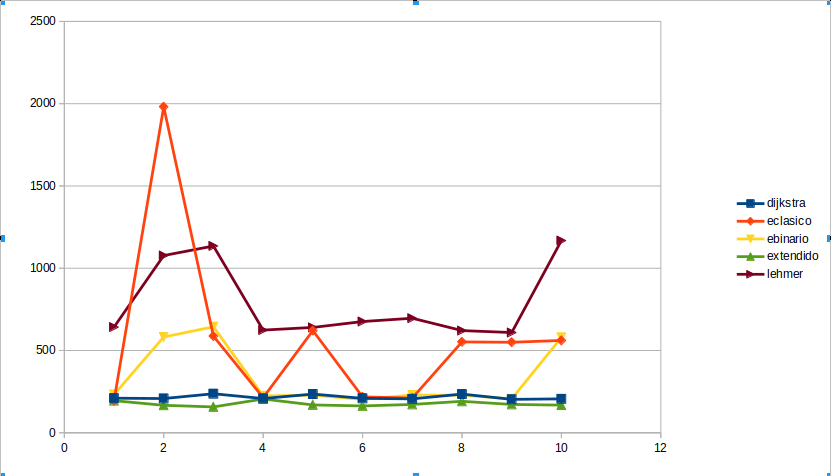
\includegraphics[scale=0.4]{pictures/32bits.png}
 % 32bits.png: 0x0 pixel, 300dpi, 0.00x0.00 cm, bb=
% \caption{Tiempo de ejecución de 32-Bits}
% \label{fig:1}
%\end{figure}



%\begin{figure}[h]
% \centering
% 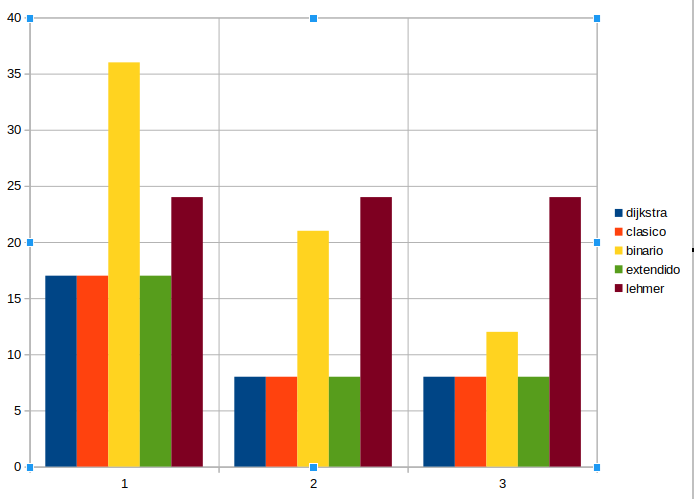
\includegraphics[scale=0.4]{pictures/iteracion.png}
 % iteracion.png: 0x0 pixel, 300dpi, 0.00x0.00 cm, bb=
% \caption{Nro de Iteraciones en 32, 16 y 8 bits}
% \label{fig:2}
%\end{figure}


\section{Comparacion de Tiempo de ejecucion}
\begin{table}[H]
\label{tablax}
\begin{center}
\begin{tabular}{|c|c|c|}
\hline 
i&a&b \\
\hline
1&938492342349723492374234723&6823234234232423234\\\hline
2&548674568475645867&534653645634\\\hline
3&2323423324&242342\\\hline
4&23423&2342\\\hline
5&234&123\\\hline
\end{tabular}
\end{center}
\caption{comparacion de tiempo}
\end{table}

\begin{figure}
    \centering
    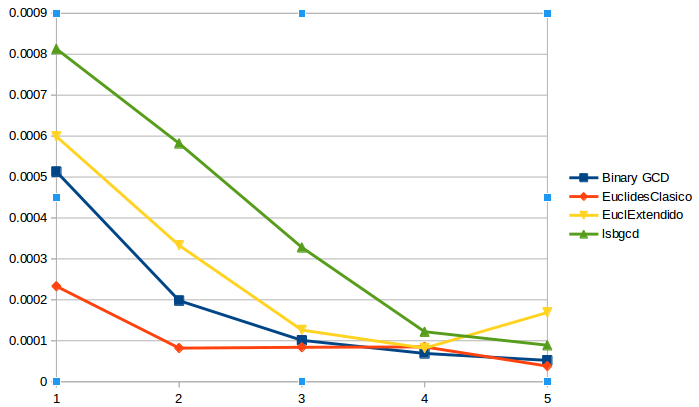
\includegraphics[scale=0.4]{pictures/dispersion.png}
    \caption{Caption conparacion de tiempo }
    
    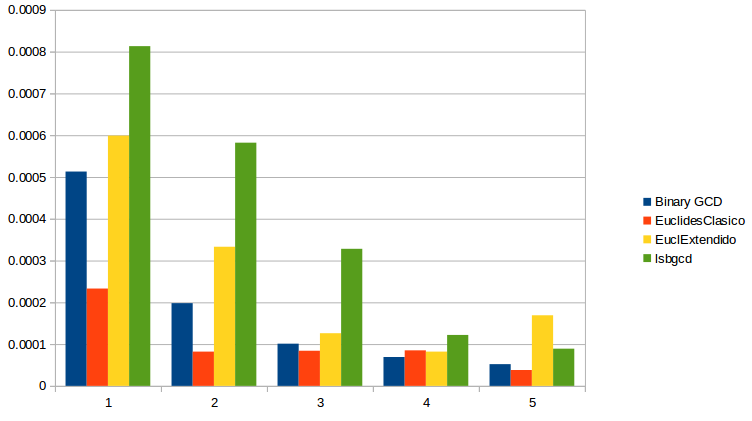
\includegraphics[scale=0.4]{pictures/barras.png}
    \caption{Caption comparacion de tiempo}
    
    \label{fig:my_label}
\end{figure}

%\begin{figure}[h]
% \centering
% 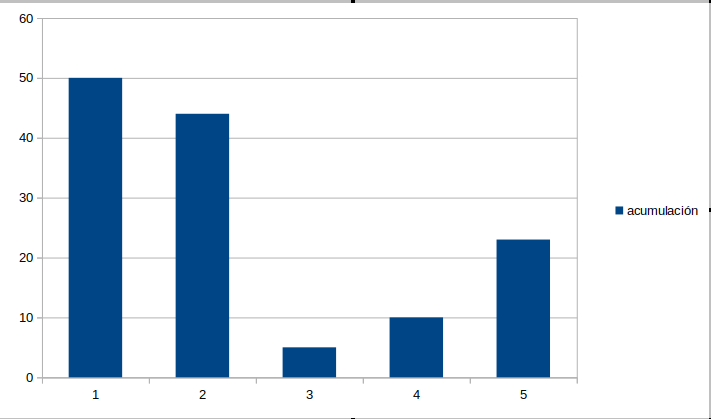
\includegraphics[scale=0.4]{pictures/acmulac.png}
 % acmulac.png: 0x0 pixel, 300dpi, 0.00x0.00 cm, bb=
% \caption{Acumulación de variable de todos los algoritmos}
% \label{fig:3}
%\end{figure}

%comparacion
%\include{suport/biogra}
%\include{conclu}

\appendix
%% Cap'itulos incluidos despues del comando \appendix aparecen como ap'endices
%% de la tesis.
%\include{apendiceA}
%\include{apendiceB}
%\include{apendiceC}

%% Incluir la bibliograf'ia. Mirar el archivo "biblio.bib" para m'as detales
%% y un ejemplo.
\nocite{*}
\bibliographystyle{plain}
\bibliography{suport/biblio} 

\end{document}
